\documentclass[11pt, a4paper, titlepage, oneside]{scrbook}

\usepackage{../Tarc/Tarc}
\usepackage{../Tarc/Tarc-private}
\graphicspath{{immagini/}}

\title{Algoritmi II}
\author{Lorenzo Ferraro}
\date{\today}
\setDegree{Informatica}

\begin{document}

\frontmatter
\SapienzaCoverItalianoTriennale
\InfoSegnalazioni

\tableofcontents

\mainmatter

\chapter{Grafi e Algoritmi sui grafi}

\section{Introduzione ai grafi}

\begin{Definizione}[Grafo]
\label{def-grafo}
Un \textbf{grafo} è una coppia ordinata \textbf{G = (V,E)} dove V è l'insieme dei \textbf{nodi} (o vertici), mentre E è l'insieme degli \textbf{archi} che collegano due vertici. 
\end{Definizione}

In questi appunti guarderemo a grafi senza loop (ossia senza archi che collegano un nodo a sè stesso) e senza archi paralleli (ossia grafi che non hanno due o più archi uguali).

\begin{minipage}[c]{0.15\textwidth}
\centering
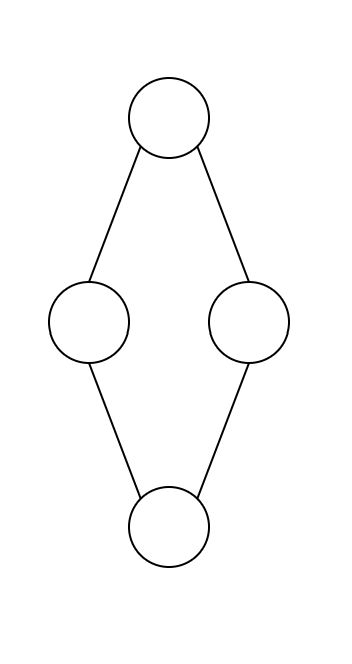
\includegraphics[width=1\textwidth, valign=t]{Grafo base.png}
\end{minipage}\hfill
\begin{minipage}[c]{0.80\textwidth}
Questo è l'esempio più classico di grafo: i nodi sono i pallini, che sono collegati da delle linee che rappresentano gli archi.
\end{minipage}

\begin{minipage}[c]{0.15\textwidth}
\centering
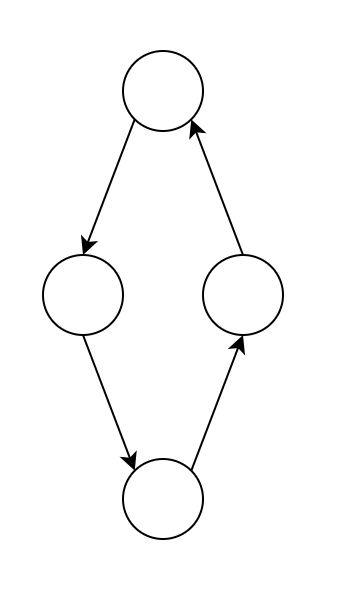
\includegraphics[width=1\textwidth, valign=t]{Grafo base frecce.png}
\end{minipage}\hfill
\begin{minipage}[c]{0.80\textwidth}
Gli archi possono avere anche un orientamento, e se tutti gli archi lo hanno diciamo che il grafo è \textbf{orientato}, come il grafo qui a sinistra. In questo caso è possibile avere due archi differenti tra due nodi x e y, ma devono avere la freccia invertita (ossia uno deve portare da x a y e l'altro da y a x). 
\end{minipage}

\begin{Proprieta}[Archi]
\label{prop-archi}
Preso un arco \textbf{f} da x a x, diciamo che
\begin{itemize}
    \item f è \textbf{incidente} a x e y
    \item x è \textbf{adiacente} a y ($\bm{x \sim y}$)
\end{itemize}
\end{Proprieta}

\begin{Definizione}[Grado di un vertice]
\label{def-grado-vertice}
Il \textbf{grado di un vertice} x ($\bm{\deg(x)}$)è il \textbf{numero di archi incidenti} ad esso.
\end{Definizione}

Nei due esempi visti prima, il grado di ogni vertice era 2.

\section{Problema dei ponti di Konisberg}

Il problema dei ponti di Konisberg è uno dei problemi logico-matematici più famosi. 

\begin{minipage}[c]{0.35\textwidth}
\centering
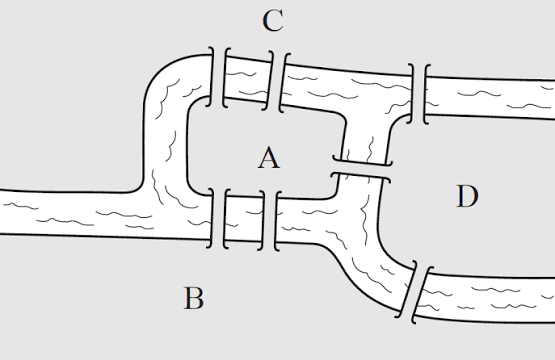
\includegraphics[width=0.7\textwidth, valign=t]{Ponti di Konisberg.png}
\end{minipage}\hfill
\begin{minipage}[c]{0.60\textwidth}
La domanda è semplice: con la seguente disposizione di ponti, è possibile attraversarli tutti una volta sola e tornare al punto di partenza?
\end{minipage}

Questo classico quesito è risolvibile usando i grafi. Infatti, possiamo schematizzarlo in questo modo:

\begin{figure}[H]
\centering
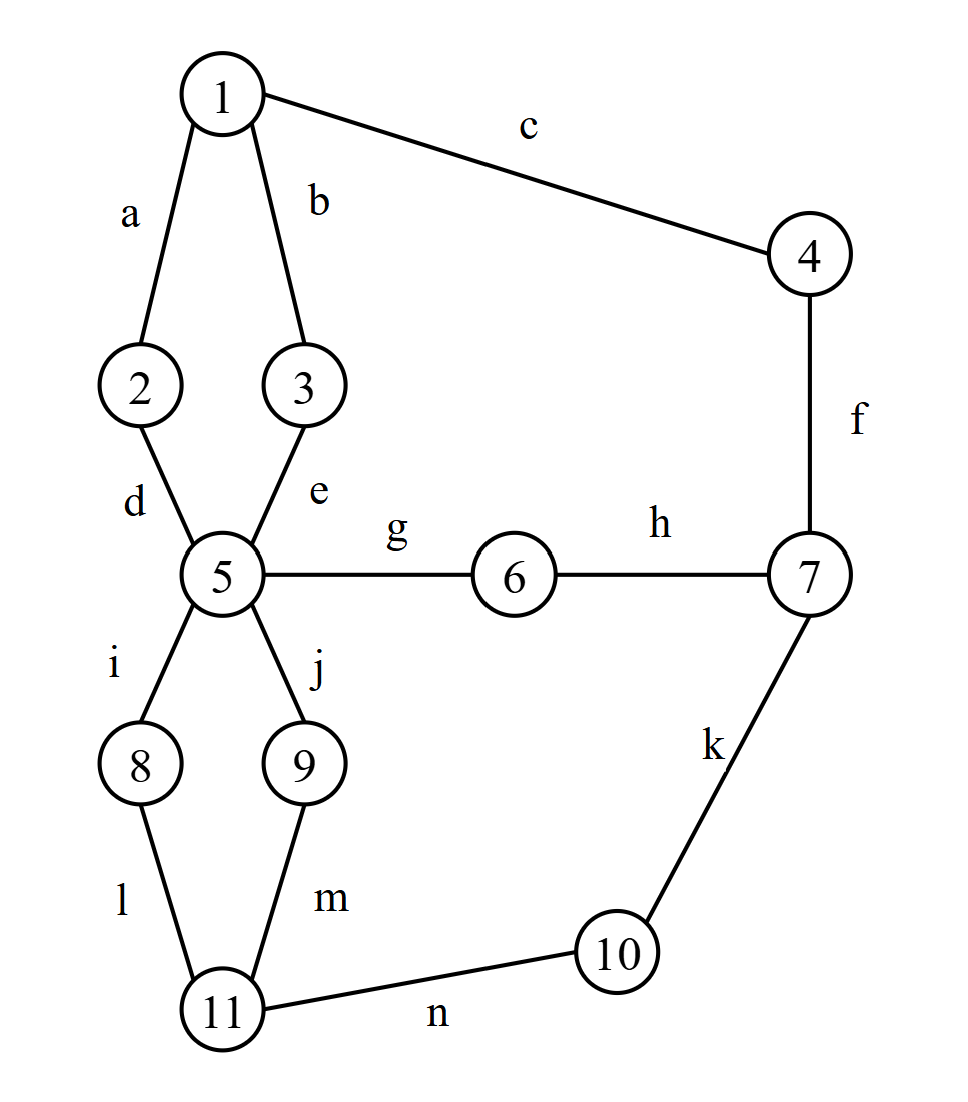
\includegraphics[width=0.3\textwidth]{Ponti di Konisberg grafi.png}
\end{figure}

\begin{Definizione}[Passeggiata]
\label{def-passeggiata}
Una \textbf{passeggiata} in un grafo è una \textbf{sequenza} del tipo $v_0 e_0 v_1 e_1 \ldots v_n e_n$, dove $v_i$ e $v_{i+1}$ indicano due vertici collegati dall'arco $e_i$. \\
Una passeggiata è detta \textbf{chiusa} se $\bm{v_0 = v_n}$.
\end{Definizione}

Una passeggiata possibile nel grafo qui sopra ad esempio è "1 a 2 d 5 i 8 l 11 n 10 k 7".

Per risolvere il problema dei ponti di Konisberg bisogna saper rispondere alla domanda "Quand'è che è esiste una passeggiata chiusa in un grafo che contiene tutti gli archi presenti una volta sola?". La risposta è che \textbf{qualsiasi grafo con almeno un nodo x tale che} $\bm{\deg(x) \% 2 = 1}$ (ossia il cui grado è dispari) \textbf{non ammette una passeggiata di questo tipo}. Nel nostro caso, quindi, il problema è irrisolvibile: infatti sia il nodo 1, 5, 7 e 11 hanno un grado dispari. Ma se fossero tutti pari? Non è comunque detto. 

\begin{minipage}[c]{0.15\textwidth}
\centering
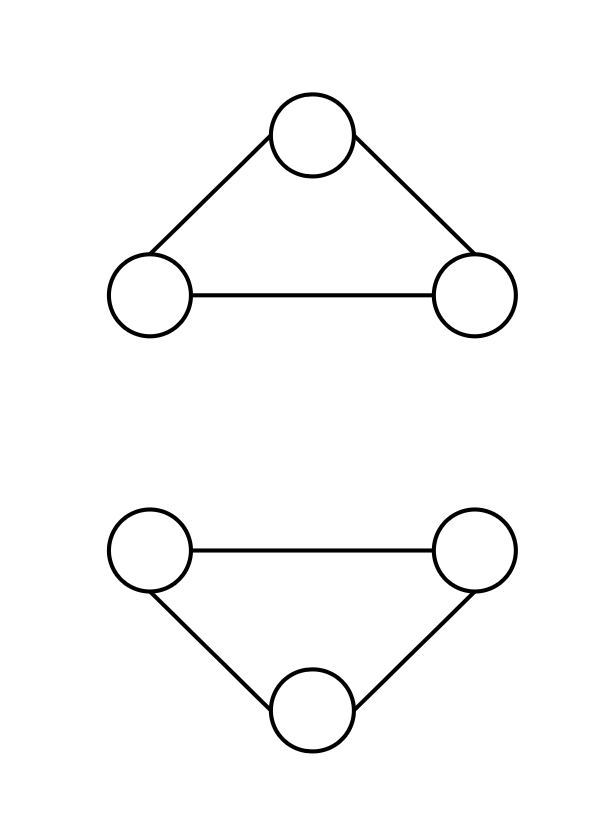
\includegraphics[width=1\textwidth, valign=t]{Grafo non connesso.png}
\end{minipage}\hfill
\begin{minipage}[c]{0.80\textwidth}
In questo caso, infatti, nonostante tutti i nodi siano di grado 2 quindi pari, la risposta al problema è comuqnue no. È infatti comuqnue necessario che il grafo sia \textbf{connesso}.
\end{minipage}

\begin{Definizione}[Grafo connesso]
\label{def-grafo-connesso}
Un grafo si dice \textbf{connesso} se per ogni coppia di vertici x e y esiste una passeggiata che porti da x a y.
\end{Definizione}

\begin{Proposizione}[]
\label{propos-problmea-ponti}
Esiste una passeggiata chiusa che contiene tutti gli archi del grafo una sola \mbox{volta $\iff$ ogni vertice} ha grado pari e il grafo è chiuso.
\end{Proposizione}

\section{Rappresentare i grafi}

\begin{minipage}[c]{0.70\textwidth}
Vedremo ora due modi differenti per rappresentare questo grafo:
\end{minipage}\hfill
\begin{minipage}[c]{0.25\textwidth}
\centering
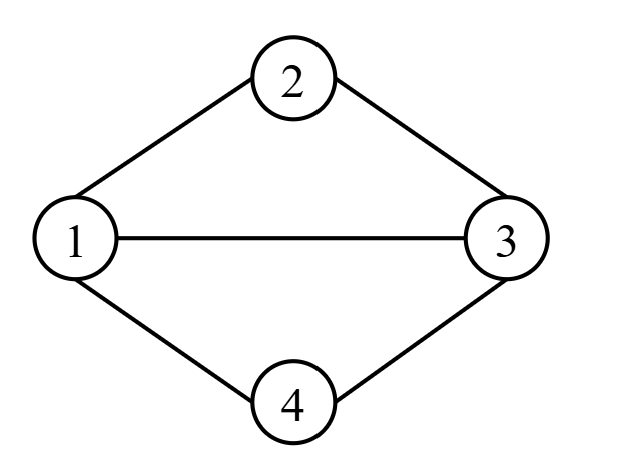
\includegraphics[width=1\textwidth, valign=t]{Grafo rappresentazione.png}
\end{minipage}

\begin{Definizione}[Matrice di adiacenze]
\label{def-matrici-di-adiacenze}
Si prende una matrice $M$ di dimensione $n \times n$ (dove $n = \# V$) tale che 
\[
\bm{m_{ij}} =
\begin{cases}
\bm{1} & \textbf{se } \bm{x \sim y} \\
\bm{0} & \textbf{altrimenti} 
\end{cases}
\]
\end{Definizione}

Nel nostro caso quindi abbiamo una matrice del tipo 
\[
\raisebox{-0.9em}{$M \,=\,$}\,
\begin{array}{@{}c@{\hspace{2pt}}c@{}}
   & \begin{array}{cccc} 1 & 2 & 3 & 4 \end{array} \\[2pt]
  \begin{array}{c} 1\\2\\3\\4 \end{array}
  &
  \left[
  \begin{array}{cccc}
    0 & 1 & 1 & 1 \\
    1 & 0 & 1 & 0 \\
    1 & 1 & 0 & 1 \\
    1 & 0 & 1 & 0
  \end{array}
  \right]
\end{array}
\]

Questa matrice, dato che non abbiamo loop nei grafi, avrà sempre la diagonale principale composta solo da 0.

\begin{Proposizione}[]
\label{propos-matrice-speculare}
Se il grafo non è diretto, la matrice di adiacenze sarà \textbf{speculare}.
\end{Proposizione}

\begin{Proprieta}[Costi computazionali matrice di adiacenze]
\label{prop-costi-matrice-adiacenze}
\begin{itemize}
    \item \textbf{Memorizzazione del grafo}: $\bm{\Theta(n^2)}$ (spaziale)
    \item \textbf{Visita del grafo}: $\bm{\Theta(n^2)}$ 
    \item \textbf{Verificare se} $\bm{i \sim j}$: $\bm{\Theta(1)}$
    \item \textbf{Preso un nodo x, calcolare} $\bm{\det(x)}$: $\bm{\Theta(n)}$
\end{itemize}
\end{Proprieta}

\begin{Definizione}[Lista di adiacenza]
\label{def-lista-adiacenze}
Si prende un'array di dimensione n, e a ogni posizione i dell'array si punta ad una \textbf{lista puntata con tutti i vicini del nodo i-esimo}.
\end{Definizione}

Nel nostro caso abbiamo quindi uno schema del tipo
\[
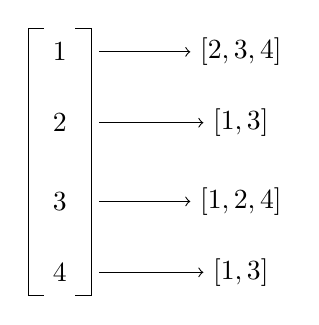
\begin{tikzpicture}[baseline={([yshift=-0.6ex]current bounding box.center)}]

  \node (n1) at (0,2.9) {$1$};
  \node (n2) at (0,2) {$2$};
  \node (n3) at (0,1) {$3$};
  \node (n4) at (0,0.1) {$4$};

  \draw (-0.2,3.2) -- (-0.4,3.2) -- (-0.4,-0.2) -- (-0.2,-0.2);
  \draw (0.2,3.2) -- (0.4,3.2) -- (0.4,-0.2) -- (0.2,-0.2);

  \node (l1) at (2.3,2.9) {$[2,3,4]$};
  \node (l2) at (2.3,2) {$[1,3]$};
  \node (l3) at (2.3,1) {$[1,2,4]$};
  \node (l4) at (2.3,0.1) {$[1,3]$};

  \draw[->] (0.5,2.9) to[out=0,in=180] (l1.west);
  \draw[->] (0.5,2)   to[out=0,in=180] (l2.west);
  \draw[->] (0.5,1)   to[out=0,in=180] (l3.west);
  \draw[->] (0.5,0.1) to[out=0,in=180] (l4.west);

\end{tikzpicture}
\]

\begin{Proprieta}[Costi computazionali lista di adiacenze]
\label{prop-costi-lista-adiacenze}
\begin{itemize}
    \item \textbf{Memorizzazione del grafo}: $\bm{\Theta(n + m)}$ (spaziale), dove $m = \# E$
    \item \textbf{Visita del grafo}: $\bm{\Theta(n+m)}$
    \item \textbf{Verificare se} $\bm{i \sim j}$: $\textbf{O}\bm{(\min(\deg(i), \deg(j)))}$
    \item \textbf{Preso un nodo x, calcolare} $\bm{\det(x)}$: $\bm{\deg(x)}$
\end{itemize}
\end{Proprieta}

In realtà, per la memorizzazione e la visita avremmo un costo pari a $\Theta(n + \sum_{v \in V} \deg(v))$, ma dato che $\Theta(n + \sum_{v \in V} \deg(v)) = \Theta(n + 2m) = \Theta(n+m)$ non abbiamo problemi.

Per i grafi diretti, invece, ci sono 3 possibilità:
\begin{enumerate}
    \item Le liste di adiacenze hanno solo i nodi in entrata
    \item Le liste di adiacenze hanno solo i nodi in uscita
    \item Ci sono due liste di adiacenze, una per i nodi in entrata e una per quelli in uscita
\end{enumerate}

Tutti e 3 i modi sono perfettamente funzionanti. Vediamo con un esempio perché.

\begin{figure}[H]
\centering
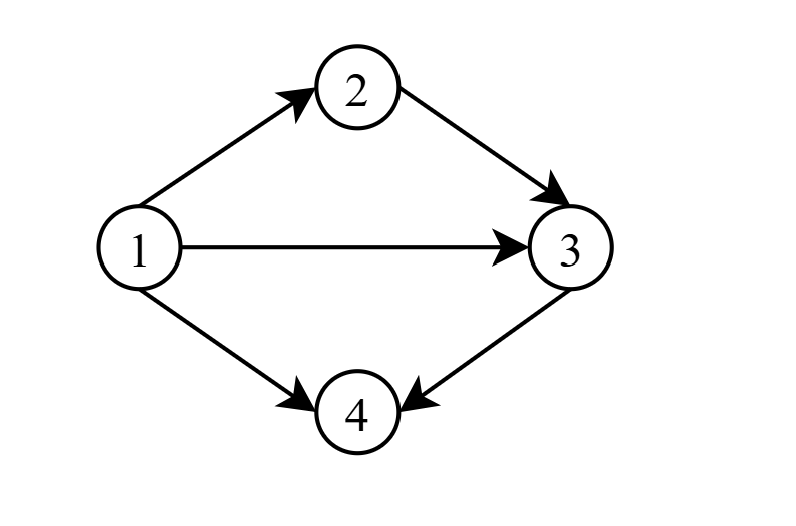
\includegraphics[width=0.5\textwidth]{Grafo diretto liste di adiacenze.png}
\end{figure}

Se usiamo le liste di adiacenza con solo i valori in entrata, allora avremo uno schema del tipo
\[
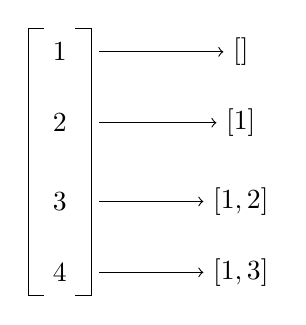
\begin{tikzpicture}[baseline={([yshift=-0.6ex]current bounding box.center)}]

  \node (n1) at (0,2.9) {$1$};
  \node (n2) at (0,2) {$2$};
  \node (n3) at (0,1) {$3$};
  \node (n4) at (0,0.1) {$4$};

  \draw (-0.2,3.2) -- (-0.4,3.2) -- (-0.4,-0.2) -- (-0.2,-0.2);
  \draw (0.2,3.2) -- (0.4,3.2) -- (0.4,-0.2) -- (0.2,-0.2);

  \node (l1) at (2.3,2.9) {$[]$};
  \node (l2) at (2.3,2) {$[1]$};
  \node (l3) at (2.3,1) {$[1,2]$};
  \node (l4) at (2.3,0.1) {$[1,3]$};

  \draw[->] (0.5,2.9) to[out=0,in=180] (l1.west);
  \draw[->] (0.5,2)   to[out=0,in=180] (l2.west);
  \draw[->] (0.5,1)   to[out=0,in=180] (l3.west);
  \draw[->] (0.5,0.1) to[out=0,in=180] (l4.west);

\end{tikzpicture}
\]

mentre quelle con solo valori in output saranno del tipo

\[
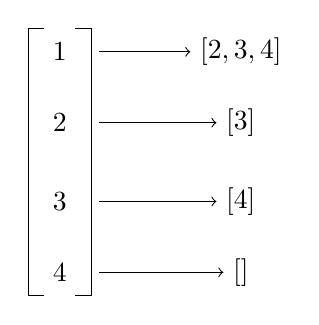
\begin{tikzpicture}[baseline={([yshift=-0.6ex]current bounding box.center)}]

  \node (n1) at (0,2.9) {$1$};
  \node (n2) at (0,2) {$2$};
  \node (n3) at (0,1) {$3$};
  \node (n4) at (0,0.1) {$4$};

  \draw (-0.2,3.2) -- (-0.4,3.2) -- (-0.4,-0.2) -- (-0.2,-0.2);
  \draw (0.2,3.2) -- (0.4,3.2) -- (0.4,-0.2) -- (0.2,-0.2);

  \node (l1) at (2.3,2.9) {$[2,3,4]$};
  \node (l2) at (2.3,2) {$[3]$};
  \node (l3) at (2.3,1) {$[4]$};
  \node (l4) at (2.3,0.1) {$[]$};

  \draw[->] (0.5,2.9) to[out=0,in=180] (l1.west);
  \draw[->] (0.5,2)   to[out=0,in=180] (l2.west);
  \draw[->] (0.5,1)   to[out=0,in=180] (l3.west);
  \draw[->] (0.5,0.1) to[out=0,in=180] (l4.west);

\end{tikzpicture}
\]

In entrambi i casi, però, non stiamo perdendo informazioni sul grafo: infatti è possibile da queste liste ricreare il grafo da cui vengono senza alcun problema.

\section{Cicli}

\begin{Definizione}[Cammino]
\label{def-cammino}
Un \textbf{cammino} è una passeggiata che \textbf{non ripete i vertici}.
\end{Definizione}

\begin{Proposizione}[]
\label{propos-cammino}
Presi due nodi x e y, esiste un cammino da x a y $\iff$ esiste una passeggiata da x a y.
\end{Proposizione}

\Dimostrazione \nopagebreak

\begin{enumerate}[label=\arabic*°]
    \item Esiste un cammino da x a y $\implies$ esiste una passeggiata da x a y \\
    È ovvio, dato che un cammino è una passeggiata. $\blacksquare$
    \item Esiste un cammino da x a y $\impliedby$ esiste una passeggiata da x a y \\
    Prendiamo la passeggiata di lunghezza minima tra x e y, e ipotizziamo per assurdo che non sia un cammino. Dunque sicuramente esiste un nodo che viene ripetuto, ossia esistono due indici $i < j$ tali che $v_i = v_j$. Possiamo allora tagliare il percorso che porta da $v_i$ di nuovo a sè stesso, dato che stiamo inutilmente allungando il giro. Ma così staremmo accorciando la passeggiata, che abbiamo detto essere di lunghezza minima. Abbiamo quindi trovato un assurdo, dunque abbiamo trovato che la passeggiata più corta è un cammino da x a y. $\blacksquare$
\end{enumerate}

\begin{Definizione}[Ciclo]
\label{def-ciclo}
Un \textbf{ciclo} è un grafo connesso dove ogni vertice è di grado 2.
\end{Definizione}

\subsection{Problema sui cicli}

"Dato un grafo dove ogni nodo x ha $\deg(x) \geq 2$, trovare un ciclo". Proviamo a studiare un algoritmo per risolvere questo problema.

Scegliamo un nodo di partenza x. Camminiamo lungo il grafo spondandoci sempre su un vicino diverso dal quale siamo arrivati (il che è possibile dato che $\deg(x) \geq 2$). Prima o poi troveremo un vicino già visitato. in quel momento il nodo su cui ci troveremo avrà due vicini già visitati, il che significa che siamo arrivati ad un ciclo.

\begin{lstlisting}[style=Python]
def trovaCiclo(G):
    L = lista vuota
    x = nodo qualsiasi con grado 2
    L.append(x)
    current = x
    next = x.neighbors[0]
    while(next not in L):
        L.append(next)
        if next.neighbors[0] == current:
            u = next.neighbors[1]
        else:
            u = next.neighbors[0]
        current = next
        next = u
    while L[0] != next:
        L.remove(L[0])
    return L
\end{lstlisting}

L'ultimo while è fondamentale perché rimuove tutti i nodi che non fanno parte del ciclo.

Vediamo con un esempio grafico perché questo algoritmo funziona, studiando il grafo
\begin{figure}[H]
\centering
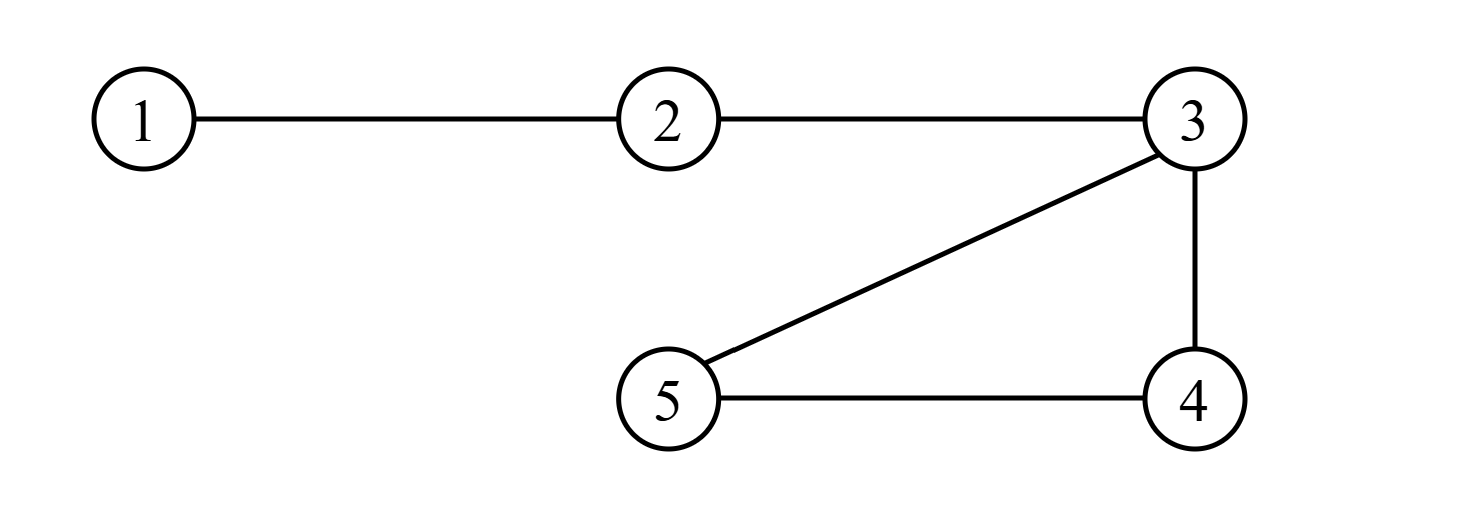
\includegraphics[width=0.6\textwidth]{Problema cicli.png}
\end{figure}

Iniziamo con \code{L = [2]}, \code{current = 2} e \code{next = 3}. Dopo il primo ciclo avremo \code{L = [2,3]}, \code{current = 3} e \code{next = 4}. Dopo il secondo ciclo avremo \code{L = [2,3,4]}, \code{current = 4} e \code{next = 5}. Dopo il terzo ciclo avremo \code{L = [2,3,4,5]}, \code{current = 5} e \code{next = 3}. Dato che ora \code{next} è in \code{L}, usciamo dal ciclo. Nel secondo while eliminiamo 2, e dunque rimane \code{L = [3,4,5]}, che è proprio il ciclo nel grafo. 

Questa versione, però, non è la più efficiente. Infatti, controllare che un elemento non sia in una lista non ordinata ha un costo $\O(n)$, dunque, dato che il primo while è eseguito n volte, arriviamo ad un costo in $\O(n^2)$. Vediamo un'altra versione più efficiente.

\begin{lstlisting}[style=Python]
def trovaCicloEfficiente(G):
    L = lista vuota
    Vis = [0] * n
    x = nodo qualsiasi con grado 2
    L.append(x)
    Vis[x] = 1
    current = x
    next = x.neighbors[0]
    while Vis[next] == 0:
        L.append(next)
        Vis[next] = 1
        if next.neighbors[0] == current:
            u = next.neighbors[1]
        else:
            u = next.neighbors[0]
        current = next
        next = u
    while L[0] != next:
        L.remove(L[0])
    return L
\end{lstlisting}

In questo caso usiamo quindi un array di supporto dove controlliamo se un nodo è già stato visitato o meno, riducendo il controllo della condizione del while da $\O(n)$ a $\O(1)$, abbassando quindi il costo temporale a $\textbf{O}\bm{(n)}$. Il costo spaziale invece rimane identico in entrambi i casi: $\textbf{O}\bm{(n)}$.


\end{document}